\section{Lupus disease prediction}

This experiment involves real data gathered by ``Lupus Clinic'', Reumatologia, Università Sapienza, Roma. The data consists in 413 patients. It is available the records of the visits that every patience has done over time. For an in-depth description of the data we refer the reader to the work of Francesco Morelli, that served as starting point of our work. In his thesis, ``Tecniche di apprendimento automatico per la classificazione di pazienti affetti da Lupus'', he performed an analysis of the data which does not take into account the history of the patience: only the first visit of each patience is considered with the aim to classify a patience as affected or unaffected by the disease at the time of the visit. This analysis led also to the identification of a subset\footnote{The subset of selected features is [Hashimoto, APS , npsle, arterialthrombosis, MyasteniaGravis, FM, age] over the whole set [ APS, DNA, FM, Hashimoto, MyasteniaGravis, SdS, age, arterialthrombosis, arthritis, c3level, c4level, dislipidemia, hcv, hematological, hypertension, hypothyroidism, kidney, mthfr, npsle, pregnancypathology, serositis, sex, skinrash, sledai2kInferred].} of features which appear to be the most relevant for the prediction. Our goal is slightly different: we aim to predict whether a patience will develop the lupus disease before it is evident from organic damage, i.e. when the SDI (systemic damage index) is zero). This is done considering not only the first visit of a patience but his complete history.

For the purpose of this thesis, the important things to underline are essentially two. The first one is that,  although each visit is described by a fixed number real and binary features, the number of visits  is not the same for each patience. RNNs then emerges as one of few models suitable for such a task. The other important thing to notice is that the visits are not equally spaced in time; they can be distanced by a month as by a few years. This is an important difference with all of the tasks considered until now. Let us think for example of the polyphonic music prediction where each song is split in equally spaced time beats.

In the experiments we used as \textbf{positive} examples all the patients which are negative at the first visit but results positive in later visits (i.e. we excluded completely all the patients which are positive from the first visit). We used as training sequences only the visits in which the patients has zero SDI .
For the \textbf{negative} examples we choose only the patients which satisfy some temporal constraints controlled by user-defined parameters. The first requirement is for the recorded history of a patience to be long enough to be able to leave out the last part of it from the training sequence. This ensures that we train the model to give a prediction valid\footnote{Contrarily to a positive patience who cannot become negative once he has positive SDI, for negative patients there is always the possibility to result positive in the future. This suggest to restrict the prediction to a span of years and use as negatives in the training process only the patience which result negative for that period of time.}, at least, for such given amount of time. We measured this time (in years) with the parameter \texttt{upper span age}.  We then require the remaining part of the visits (which are the only ones used in the training sequence) to cover a sufficiently long period of time with the parameter (in years) \texttt{lower span age} and to be composed by at least \texttt{min visits} number of visits. This last two constraints are needed to filter out the examples which do not have enough information: if the network has to understand the data from its evolution over time, we should have sufficiently many recordings for a sufficient amount of time.

\tikzstyle{rnn_style}=[shorten >=1pt,auto,node distance=0.5cm,
thick,
sdi/.style={rectangle,fill=white!50,node distance=0.7cm, draw=none,minimum size=0.5cm,font=\sffamily\normalsize},
missing/.style={circle,fill=white!50,draw,minimum size=0.7cm,font=\sffamily\Huge\bfseries},
label/.style={node distance=0.9cm and 4cm,rectangle,fill=white!50,draw=none,minimum size=0.7cm,font=\sffamily\normalsize},
thick_edge/.style={line width=1.2pt},
thin_edge/.style={line width=0.5pt}
]
\begin{figure}[h]
	\centering
	\begin{tikzpicture}[rnn_style]
	
	%SDI column
	
	\node[sdi]    (x1)[]   {$0$};
	\node[sdi]    (x2)[above of=x1]   {$0$};
	\node[sdi]    (x3)[above of=x2]   {$0$};
	\node[sdi]    (x4)[above of=x3]   {$0$};
	\node[sdi]    (x5)[above of=x4]   {$0$};
	\node[sdi]    (x6)[above of=x5]   {$0$};
	\node[sdi]    (x7)[above of=x6]   {$0$};
	\node[sdi]    (x8)[above of=x7]   {$0$};
	\node[label]  (sdiLabel)[above of = x8] {SDI};
	
	%AGE column
	
	\node[sdi]    (y1)[right =0.5cm of x1]   {$20$};
	\node[sdi]    (y2)[above of=y1]   {$21$};
	\node[sdi]    (y3)[above of=y2]   {$22$};
	\node[sdi]    (y4)[above of=y3]   {$25$};
	\node[sdi]    (y5)[above of=y4]   {$30$};
	\node[sdi]    (y6)[above of=y5]   {$35$};
	\node[sdi]    (y7)[above of=y6]   {$40$};
	\node[sdi]    (y8)[above of=y7]   {$45$};
	\node[label]  (sdiLabel)[above of = y8] {AGE};
	
	\node[label] (arr) [left = 0.7cm of x5] {last training visit};
	
	\draw[decorate,decoration={brace,raise=8pt,amplitude=6pt}, thick]
	(x1.center)--(x5.center) node [black,midway,xshift=-0.7cm, align=center, text width = 3cm] {
		training visits (at least \texttt{min visits})};
	
	\draw[decorate,decoration={brace,raise=8pt,amplitude=6pt, mirror}, thick]
	(y5.center)--(y8.center) node [black,midway,xshift=3.5cm] {
		\texttt{upper span age}};
	
	\draw[decorate,decoration={brace,raise=8pt,amplitude=6pt, mirror}, thick]
	(y1.center)--(y5.center) node [black,midway,xshift=3.5cm] {
		\texttt{lower span age}};
	
	\path[->]
	(arr) edge []  node[]{} (x5);
	
	
	\end{tikzpicture}
	\caption{Example of a negative training sequence.}
	\label{fig:lupus_neg_example}
\end{figure}

We employed the following metrics to evaluate the results of the experiments:
\begin{itemize}
	\item $precision \defeq \frac{TP}{TP+FP}$,
	\item $recall(sensitivity) \defeq \frac{TP}{P}$,
	\item $specificity \defeq 	\frac{TN}{N}$,
	\item area under curve (AUC): the area under the curve obtained plotting recall and specificity varying the threshold of the classifier,
\end{itemize}
where $TP, TN, P, N$ are the true positive, true negative, number of positive and number of negatives respectively. See \cite{RocMetrics} for more details on these metrics.

We normalized all the data to lie in range (0,1). 
We used RNNs with 50 hidden units trained with SGD paired with the gradient clipping technique (learning rate 0.001 and threshold 1).

Since the number of available patients is not big enough to allow a split in train, validation and test sets, we repeated the training procedure eight times with different splits of train and test, and then we put together the predictions on the eight test sets to compute the scores. We stopped each training procedure when the AUC score on the training set was below 0.92.
 
We explored all the combination for \texttt{upper span age} in [1, 2], \texttt{lower span age} in [1, 2], \texttt{min visits} in [2, 3, 4, 5].  We repeated the experiment twice: on time with all the features and next with the subset of selected features.



\begin{table}[!h]
	\centering
	\begin{tabular}{C{1.5cm}  C{1.5cm}  c | C{2cm}  C{2cm} |  c  c}
		upper span age & lower span age & min visits & AUC all feats & AUC subset feats& pos & neg\\
		\hline
		0.8 & 0.8 & 1 & 0.63 & 0.65 & 38 & 143\\
		0.8 & 0.8 & 2 & 0.66 & 0.63 & 38 & 138\\
		0.8 & 0.8 & 3 & 0.71 & 0.67 & 38 & 124\\
		0.8 & 0.8 & 4 & 0.69 & 0.75 & 38 & 115\\
		0.8 & 0.8 & 5 & 0.74 & \textbf{0.77} & 38 & 94 \label{table:line:best_config}\\
		1.0 & 0.8 & 1 & 0.69 & 0.61 & 38 & 141\\
		1.0 & 0.8 & 2 & 0.68 & 0.60 & 38 & 133\\
		1.0 & 0.8 & 3 & 0.68 & 0.67 & 38 & 121\\
		1.0 & 0.8 & 4 & 0.69 & 0.73 & 38 & 108\\
		1.0 & 0.8 & 5 & 0.74 & 0.76 & 38 & 88\\
		2.0 & 0.8 & 1 & 0.72 & 0.68 & 38 & 99\\
		2.0 & 0.8 & 2 & 0.71 & 0.67 & 38 & 97\\
		2.0 & 0.8 & 3 & 0.73 & 0.72 & 38 & 90\\
		2.0 & 0.8 & 4 & 0.74 & 0.73 & 38 & 70\\
		2.0 & 0.8 & 5 & 0.69 & \textbf{0.77} & 38 & 48\\
		0.8 & 1.0 & 1 & 0.64 & 0.65 & 38 & 138\\
		0.8 & 1.0 & 2 & 0.69 & 0.68 & 38 & 133\\
		0.8 & 1.0 & 3 & 0.66 & 0.69 & 38 & 122\\
		0.8 & 1.0 & 4 & 0.67 & 0.69 & 38 & 114\\
		0.8 & 1.0 & 5 & 0.69 & 0.72 & 38 & 93\\
		1.0 & 1.0 & 1 & 0.67 & 0.60 & 38 & 134\\
		1.0 & 1.0 & 2 & 0.64 & 0.52 & 38 & 127\\
		1.0 & 1.0 & 3 & 0.73 & 0.68 & 38 & 118\\
		1.0 & 1.0 & 4 & 0.73 & 0.73 & 38 & 107\\
		1.0 & 1.0 & 5 & 0.70 & 0.73 & 38 & 87\\
		2.0 & 1.0 & 1 & 0.69 & 0.62 & 38 & 89\\
		2.0 & 1.0 & 2 & 0.72 & 0.59 & 38 & 87\\
		2.0 & 1.0 & 3 & 0.73 & 0.63 & 38 & 83\\
		2.0 & 1.0 & 4 & 0.74 & 0.67 & 38 & 67\\
		2.0 & 1.0 & 5 & 0.69 & 0.75 & 38 & 48\\
		0.8 & 2.0 & 1 & 0.63 & 0.72 & 38 & 97\\
		0.8 & 2.0 & 2 & 0.67 & 0.66 & 38 & 95\\
		0.8 & 2.0 & 3 & 0.70 & 0.73 & 38 & 92\\
		0.8 & 2.0 & 4 & 0.68 & 0.69 & 38 & 91\\
		0.8 & 2.0 & 5 & 0.70 & 0.76 & 38 & 83\\
		1.0 & 2.0 & 1 & 0.64 & 0.66 & 38 & 88\\
		1.0 & 2.0 & 2 & 0.64 & 0.69 & 38 & 86\\
		1.0 & 2.0 & 3 & 0.66 & 0.66 & 38 & 85\\
		1.0 & 2.0 & 4 & 0.62 & 0.71 & 38 & 84\\
		1.0 & 2.0 & 5 & 0.67 & 0.74 & 38 & 74\\
		2.0 & 2.0 & 1 & 0.64 & 0.67 & 38 & 45\\
		2.0 & 2.0 & 2 & 0.68 & 0.58 & 38 & 44\\
		2.0 & 2.0 & 3 & 0.68 & 0.67 & 38 & 43\\
		2.0 & 2.0 & 4 & 0.70 & 0.64 & 38 & 41\\
		2.0 & 2.0 & 5 & 0.66 & 0.69 & 38 & 35\\
	\end{tabular}
	\caption{AUC core for different training sets. Best score in bold.}
	\label{table:exp_res}
\end{table}


\begin{figure}[h]
	\centering
	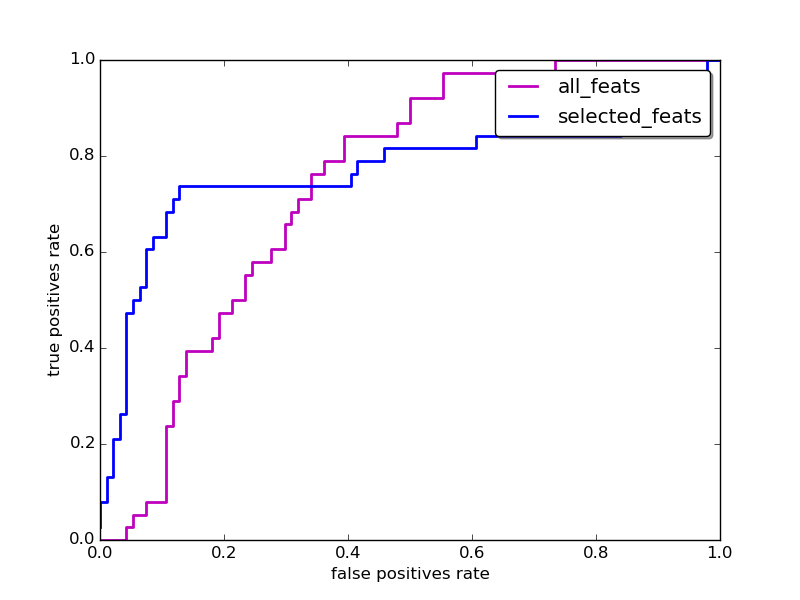
\includegraphics[width= 0.8\textwidth]{chapter4/roc_curve_comp.png}
	\caption{roc curve for models of Line \ref{table:line:best_config} of Table \ref{table:exp_res}.}
	\label{fig:roc_best}
\end{figure}

\begin{figure}[h]
	\centering
	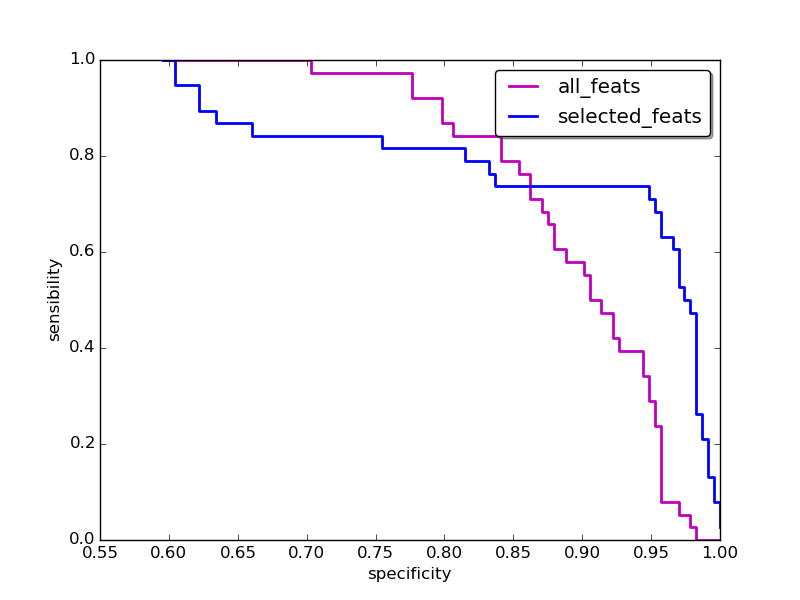
\includegraphics[width= 0.8\textwidth]{chapter4/specificity_sensitivity_comp.png}
	\caption{Sensitivity-specificity for models of Line \ref{table:line:best_config} of Table \ref{table:exp_res}.}
	\label{fig:sensitivity_specificity_best}
\end{figure}

\begin{figure}[h]
	\centering
	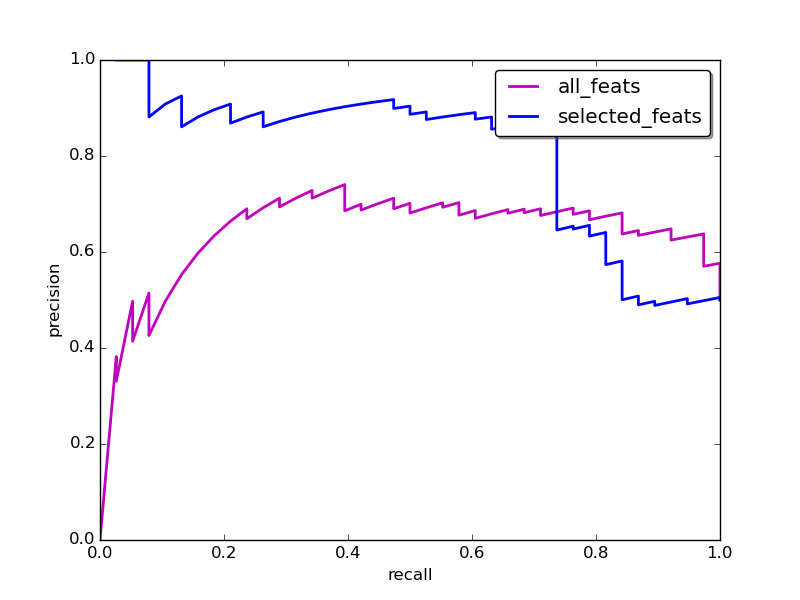
\includegraphics[width= 0.8\textwidth]{chapter4/precision_recall_comp.png}
	\caption{Precision-recall curve for models of Line \ref{table:line:best_config} of Table \ref{table:exp_res}.}
	\label{fig:precision_recall_best}
\end{figure}

From the results, shown in Table \ref{table:exp_res}, seems clear that the models trained with patients with more visits result in better AUC score. The other parameters, namely \texttt{upper span age} and \texttt{lower span age}, seems to have a little bit less influence. Moreover we notice that the better results are obtained by the models trained with the selected subset of features. In Figures \ref{fig:roc_best}, \ref{fig:sensitivity_specificity_best} and \ref{fig:precision_recall_best} are shown the plots of the roc, sensitivity-specificy and recall-precision curves for the best configuration of parameters (\texttt{upper span age}=0.8, \texttt{lower span age}=0.8 and \texttt{min visits}=5).
